%resultados_e_discussao.tex

\chapter{Resultados e discussão}

\section{Análise dos questionários de perfil de usuário}

    A FEBRACE ocorreu nos dias 17, 18 e 19 de março de 2009 e durante esse período foram aplicados questionários para alunos e professores participantes, principais usuários potenciais do sistema proposto, além de visitantes da feira. Foram respondidos 520 questionários, uma excelente amostra já que, segundo os organizadores do evento, participaram da sétima edição da FEBRACE 886 pessoas entre alunos finalistas, orientadores e coorientadores, grupo no qual se concentrou a pesquisa. Já o número de questionários respondidos por visitantes foi menor que 1\% do total, não representando uma amostra significativa desse grupo, estimado em mais de 12.000 pessoas.

  \subsection{Automação do processamento de dados coletados}
    O método escolhido para a aplicação do questionário foi em papel. Porém, com o objetivo de facilitar tanto a inserção de dados no computador quanto a compilação desses dados decidiu-se pelo uso de alguma ferramenta baseada na rede.

    A ferramenta escolhida foi o LimeSurvey, uma \textit{webapp} de código aberto que foi instalada e configurada localmente. Com ela os dados de cada questionário puderam ser inseridos de forma mais rápida e prática e, pelo fato de estar disponível \textit{online} e acessível via \textit{webrowsers}, o trabalho pôde ser mais facilmente entre os membros do grupo. Além disso, a ferramenta possibilita a geração diversas estatísticas e renderiza os respectivos gráficos. Os dados colhidos pela aplicação podem também ser exportados para diversos formatos. Essa foi a alternativa escolhida, e a análise dos dados foi realidada no \textit{software} OpenOffice Spreadsheets.

  \subsection{Análise dos dados}

    Com o intuito de levantar o perfil socioeconômico dos participantes, foi perguntado sobre o tipo de instituição a qual estão vinculados. Como se pode ver no gráfico~\ref{escola}, quase 50\% dos participantes são provenientes de escolas públicas e 15\% são de fundações educacionais, o que mostra que grande parte dos participantes são das classes baixa e média brasileira.

    \begin{grafico}
        \begin{center}
    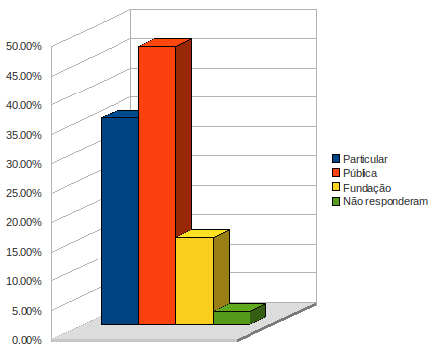
\includegraphics[width=0.7\linewidth]{arquivos/escola.png}
        \end{center}
        \caption{Tipo de escola dos participantes}
        \label{escola}
    \end{grafico}

    Para ter um perfil etário de possíveis usuários do sistema, foi feito um levantamento dos tipos de participantes que responderam ao questionário. Segundo o gráfico~\ref{participante}, cerca de 70\% dos potenciais usuários são jovens com até 25 anos.

    \begin{grafico}
        \begin{center}
    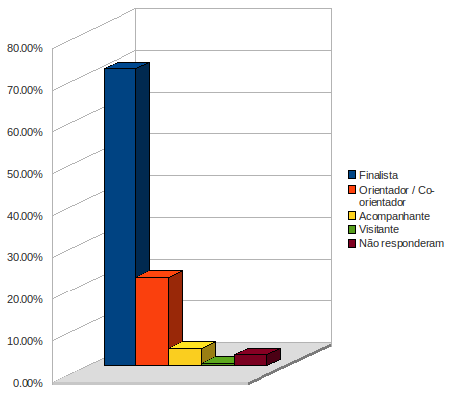
\includegraphics[width=0.7\linewidth]{arquivos/participante.png}
        \end{center}
        \caption{Tipo de participantes}
        \label{participante}
    \end{grafico}

    O gráfico~\ref{local} mostra uma compilação da frequência de uso da internet em alguns locais. Pode-se constatar algumas coisas interessantes a partir da análise desse gráfico. É provável que os 12\% dos participantes que não acessam a Internet em casa não o façam por não ter acesso devido a condições financeiras, seja acesso discado ou banda larga, e é possível que nem possuam computador em casa. Mas dentre aqueles que possuem computador e acesso a internet, pode-se perceber que quase 60\% dizem acessar a internet diaramente. Mais de 70\% dos participantes possuem acesso a Internet na escola, enquanto apenas cerca de 12\% não possuem acesso na escola, o que pode ser devido a não existir sala de informática ou à falta da conexão em si. É possível perceber que é baixa a frequencia de uso em espaços como lan houses e espaços públicos (nesse caso, foram considerados espaços públicos telecentros e bibliotecas; as escolas públicas não entraram), ou seja, menos de 10\% dos participantes fazem uso frequente desses locais para acessar a internet.

    \begin{grafico}
        \begin{center}
    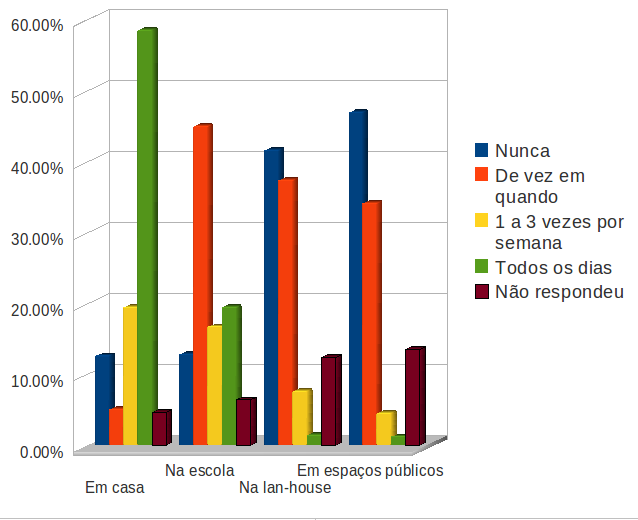
\includegraphics[width=0.7\linewidth]{arquivos/local.png}
        \end{center}
        \caption{Frequência de uso da Internet em locais}
        \label{local}
    \end{grafico}

    Quanto aos aparelhos utilizados no acesso a internet, pode-se perceber pelo gráfico~\ref{dispositivo} que a grande parcela dos acessos são feitos ainda por computadores \textit{desktop}, apesar de ter um número considerável de usuários de \textit{laptops}. Os dispositivos móveis, como celular e \textit{handhelds}, possuem uma penetração ainda baixa; apenas cerca de 30\% dos participantes dizem já terem os usados para acessar a internet, sendo que mais da metade desse valor são de acessos esporádicos (de vez em quando).

    \begin{grafico}
        \begin{center}
    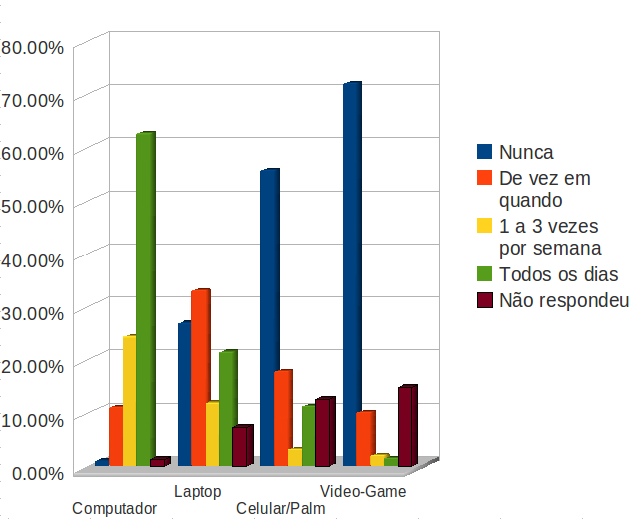
\includegraphics[width=0.7\linewidth]{arquivos/dispositivo.png}
        \end{center}
        \caption{Frequência de utilização de aparelhos para acesso a Internet}
        \label{dispositivo}
    \end{grafico}

    No gráfico~\ref{atividade}, percebe-se que o \textit{e-mail} é o serviço que os participantes acessam com maior frequência: mais de 50\% faz uso dele diariamente. O segundo serviço mais acessado diariamente são os mensageiros instantâneos, como o MSN \textit{messenger} e o GTalk, com quase 40\%  das pessoas fazendo uso diário dele. Ao contrário do que é senso comum, as redes sociais são o quarto serviço em utilização diária com apenas pouco mais de 20\% dos participantes. Como pode-se constatar jogos, blogs, fóruns e chat possuem acesso esporádico entre os participantes da FEBRACE, sendo grande a porcentagem de pessoas que dizem nunca fazer uso deles. O acesso a vídeos, apesar de esporádico (com mais de 40\% das pessoas dizendo que usam “de vez em quando"), possui uma baixa porcentagem de participantes que não fazem uso desse serviço.

    \begin{grafico}
        \begin{center}
    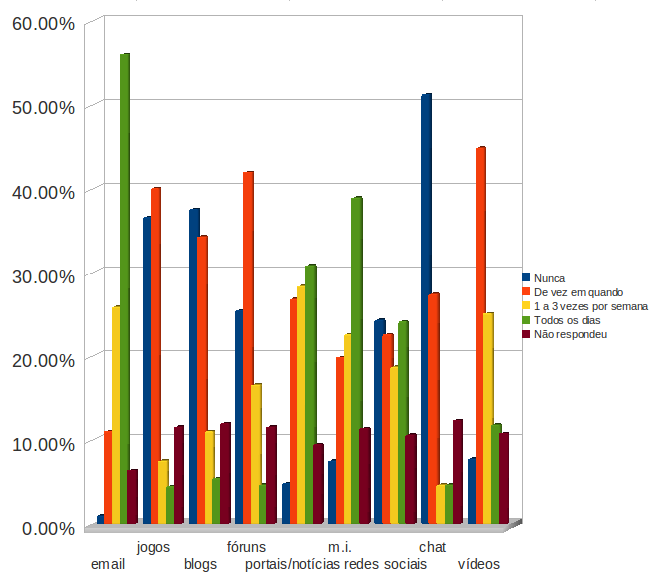
\includegraphics[width=0.7\linewidth]{arquivos/atividade.png}
        \end{center}
        \caption{Frequência de acesso a serviços na Internet}
        \label{atividade}
    \end{grafico}

    Quanto às redes sociais mais usadas, segundo o gráfico~\ref{rede_social}, mais de 75\% dos participantes possuem conta na rede social Orkut, do Google. Em todas as demais, os participantes que as possuem não chega nem aos 10\%. Cerca de 15\% dos participantes afirmam não participar de redes sociais.

    \begin{grafico}
        \begin{center}
    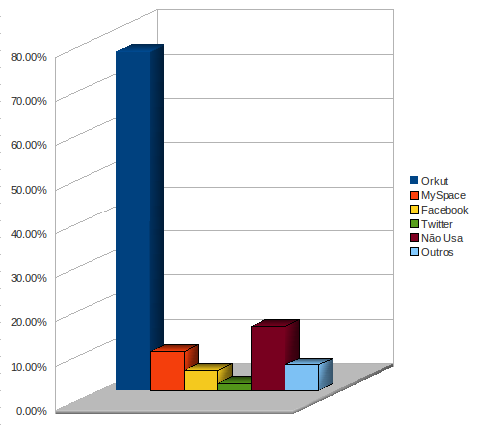
\includegraphics[width=0.7\linewidth]{arquivos/rede_social.png}
        \end{center}
        \caption{Redes Sociais mais utilizadas}
        \label{rede_social}
    \end{grafico}

    Como pode-se ver no gráfico~\ref{contato} para mais de 85\% dos participantes é importante manter contato com os demais participantes da feira após seu término. Isso reforça a idéia que um espaço para o encontro desses participantes seria muito bem vindo.

    \begin{grafico}
        \begin{center}
    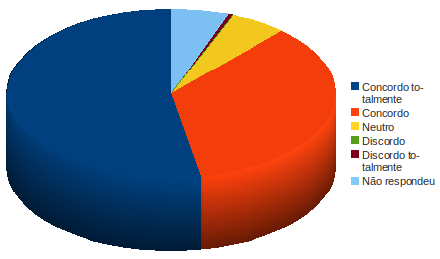
\includegraphics[width=0.7\linewidth]{arquivos/contato.png}
        \end{center}
        \caption{Participantes que acham importante poder manter contato com os outros da feira após o fim da Febrace}
        \label{contato}
    \end{grafico}

    Mais de 60\% dos participantes, de acordo com o gráfico~\ref{feira_virtual}, acham que é possível que um grupo trabalhe num mesmo projeto sem estar na mesma cidade, através do uso da Internet. Apesar desse não ser o foco do atual projeto, mostra uma potencialidade para extensão no futuro, agregando funcionalidades que apóiem essa possibilidade.

    \begin{grafico}
        \begin{center}
    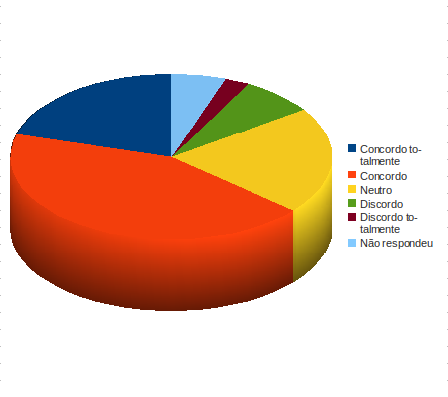
\includegraphics[width=0.7\linewidth]{arquivos/trabalho_online.png}
        \end{center}
        \caption{Participantes que acham possível um grupo trabalhar num mesmo projeto sem estar na mesma cidade, pela Internet}
        \label{trabalho_online}
    \end{grafico}

    De acordo com o gráfico~\ref{feira_virtual} mais de 60\% dos participantes acham que a idéia de uma feira de ciências virtual é interessante, enquanto apenas cerca de 10\% discordam da idéia. Isso reforça que a idéia do presente projeto apresenta relevância entre pessoas interessadas na temática.

    \begin{grafico}
        \begin{center}
    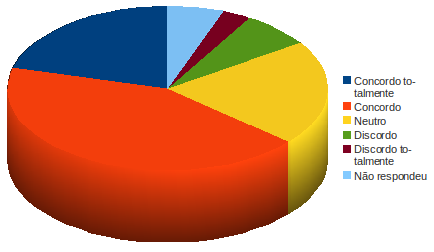
\includegraphics[width=0.7\linewidth]{arquivos/feira_virtual.png}
        \end{center}
        \caption{Participantes que acham a idéia de uma feira de ciências virtual na internet interessante}
        \label{feira_virtual}
    \end{grafico}

\section{Relato do processo de desenvolvimento}

  A adoção de metodologias ágeis em projetos universitários é ainda incomum em todo o mundo, e no Brasil em particular. Há entretanto diversas iniciativas nessa direção, conforme relatado na seção~\ref{xp_e_universidade}, e o presente trabalho visa ser uma dessas iniciativas, representando um estudo de caso da adoção da programação extrema em projeto de graduação em Engenharia. Por esse motivo, essa seção busca relatar algumas das práticas que guiaram o desenvolvimento do projeto.

  Muitas das práticas da programação extrema podem ser adotadas facilmente nas universidades para melhorar o processo de desenvolvimento de \textit{software}. Um conjunto delas, entretanto, precisa ser adaptada para o contexto acadêmico, pois foram concebidas voltadas ao contexto do desenvolvimento comercial de \textit{software}. Com base nas experiências de outros grupos que adotaram essa metodologia ágil em disciplinas de graduação, uma série de práticas do XP foram adaptadas no processo de desenvolvimento da Febrace\textsuperscript{V}. Essa seção relata as práticas de XP adotadas pela equipe, e as adaptações realizadas, quando necessárias.

  \subsection{Espaço de trabalho compartilhado virtual}
    Não foi possível dispor de um espaço de trabalho fixo para a realização das atividades referentes ao projeto. Na tentativa de suprir essa necessidade, foi feito o uso de um conjunto de ferramentas de trabalho colaborativo pela Internet, entre elas um quadro branco virtual e uma ferramenta de acompanhamento de \textit{bugs}. Mais detalhes sobre algumas dessas ferramentas foram apresentados na seção~\ref{tecnologias}.

    Essas ferramentas supriram a contento as alternativas normalmente adotadas num projeto de XP no gerenciamento de histórias e organização e planejamento da equipe.

  \subsection{Disponibilidade de tempo}
    Sendo impossível a dedicação exclusiva ao projeto, buscou-se em compensação manter um carga de trabalho semanal de 8 horas.

  \subsection{Presença do cliente}
    O papel do cliente foi designado a um pesquisador do NATE-LSI que participa da organização da Febrace, e em conjunto com ele foram escritas os cartões de histórias O cliente participou também dos \textit{Planning games}, atribuindo prioridade às histórias e definindo o conjunto de cartões a serem implementados numa iteração, e das retrospectivas, nas quais foram apresentadas a funcionalidades desenvolvidas.

  \subsection{Ciclos curtos}
    O trabalho em ciclos curtos é incentivado em XP, e o ciclo de uma semana é considerado ideal no ambiente corporativo. Mas isso se dá porque com 40 horas de trabalho semanal, um volume de trabalho grande é realizado. Como no projeto dedicou-se menos do que 25\% desse número de horas semanais, foi necessário encontrar um ciclo de tamanho adequado.

    Um ciclo de quatro semanas foi considerado, para manter a proporção de horas por ciclo de um projeto XP ideal. Um ciclo de quatro semanas é porém muito longo, e ciclos curtos são fundamentais para o acompanhamento correto do projeto. Ciclos curtos evitam atrasos, pois forçam a reflexão constante sobre o andamento do projeto, e trazem a possibilidade do replanejamento e redefinição de escopo, quando necessário. Um ciclo de quatro semanas teria possibilitado a realização de apenas dois ciclos durante o projeto, o que permitiria pouco tempo de avaliação e replanejamento.

  Tendo isso em vista, optou-se por um ciclo de desenvolvimento de duas semanas, que apresentou uma relação equilibrada entre tarefas realizadas num ciclo e ciclos realizados no projeto.

  \subsection{Retrospectivas}
    A restropectiva é uma reunião periódica na qual é avaliado o período anterior do projeto (entre aquela retrospectiva e a anterior). Nessa reunião participa toda a equipe de desenvolvimento e nela procura-se levantar coisas que deram certo naquele período, coisas que precisam ser melhoradas e idéias (desde do projeto em si até coisas referentes ao ambiente de trabalho) que possam ter surgidos durante esse período. Não há um tempo pré-determinado entre retrospectivas, mas para equipes que trabalham em período integral juntas é aconselhável que sejam quinzenais, enquanto não é ideal que demorem mais que um mês para ocorrer. Como uma adaptação ao processo, foi decidido que no caso do projeto em questão essas restrospectivas ocorreriam mensalmente.

  \subsection{Programação pareada}
    A dificuldade da prática de programação pareada em projetos acadêmicos se dá por dois motivos principais. Um é o estranhamento causado por essa prática incomum, que gera resistência de sua adoção pelos programadores. Outra são os horários fragmentados dos alunos, que nem sempre tem agendas coincidentes.

    Nesse projeto, o primeiro motivo foi rapidamente sanado, pois a resistência ao pareamento é enfraquecida nas primeiras sessões, devido aos benefícios trazidos pela prática, como redução dos erros inseridos no código e a maior rapidez na resolução de tarefas complexas. Já o problema dos horários não pode ser completamente contornado. Das oito horas semanais dedicadas ao projeto, cinco foram dedicadas à programação pareada, e demais se deram por trabalho cooperativo à distância.

  \subsection{Testes}

%  - Arquitetura
%  - Levantamento de histórias
%  - Page flow
%  - Iterações e Retrospectivas
\section{Projeto}

  A primeira fase de um projeto de XP é a fase de exploração\cite{beck04}, que abrange a tomada inicial de histórias, o levantamento inicial de aspectos relativos à arquitetura do sistema a ser desenvolvido e a escolha e familiarização com as tecnologias a serem utilizadas no projeto.

  A fase de exploração do Febrace\textsuperscript{V} ocorreu nas três primeiras semanas de abril, e nela foram realizadas as atividades descritas nas seções a seguir.

  \subsection{Levantamento inicial de Histórias}

    O planejamento em XP feito com Histórias escritas em pequenos cartões. Cada cartão é escrito pelo cliente e deve descrever uma unidade de funcionalidade, que geralmente representa um requisito funcional desejado\cite{sato07}.

    Como uma forma de especificar o sistema a ser desenvolvido durante o projeto de formatura optou-se por descrever as histórias levantadas. As histórias foram escritas em conjunto com o cliente.

    \begin{enumerate}
      \item Convite a ex-participantes \\
        Quero, como administrador do sistema, que seja enviado automaticamente um convite para participação na rede social para todos os participantes de edições anteriores da FEBRACE (cadastrados em um banco de dados legado). Caso o ex-participante crie seu perfil na rede social, o projeto dele deve ser criado automaticamente e associado a ele.
      \item Autenticação no sistema \\
        Quero, como usuário, acessar a página inicial com meu e-mail e senha para me autenticar no sistema. Caso esqueça minha senha, quero informar o sistema e pedir que envie uma nova senha para meu e-mail. Se não for um usuário registrado, quero que me seja apresentada a tela de cadastro de novo usuário.
      \item Cadastro de Usuário \\
        Quero poder criar um perfil no sistema através de cadastro no sistema fornecendo um e-mail válido e uma senha para o acesso.
      \item Edição de Perfil \\
        Quero, como usuário registrado, poder editar a página de meu perfil pessoal, alterando, inserindo e excluindo os dados lá presentes, e escolhendo quais usuários podem ter acesso a determinadas informações minhas.
      \item Visualização de Perfil \\
        Quero, como usuário, poder visualizar meu perfil e de meus amigos, bem como, via sistema de busca, visualizar os perfis de quem o permita a qualquer usuário.
      \item Cancelamento de Cadastro \\
        Quero, como usuário, poder quando assim desejar cancelar meu cadastro do sistema.
      \item Visualização de Projeto \\
        Quero, como usuário, ver as informações de cada projeto, como seu nome e resumo, sua área do conhecimento, participantes e demais informações relevantes.
      \item Visualização de Participantes de um projeto \\
        Quero, como usuário, ver na página de um projeto quais são seus participantes, e ter acesso a seus perfis. Gostaria de saber também qual seu papel na Feira (estudante, orientador, etc.) e a instituição a qual pertence.
      \item Visualização de Vídeo de um projeto \\
        Quero, como usuário, poder ver na página de um projeto, quando disponível, seu vídeo oficial, feito na própria FEBRACE, hospedado em um site dedicado como a IPTV-USP ou o Youtube.
      \item Visualização de prêmios de um projeto \\
        Quero, como usuário, saber quais prêmios foram ganhos por algum projeto na edição da feira em que participou. Quero também poder acessar mais informações sobre esses prêmios.
      \item Edição dos Conteúdos de um projeto \\
        Quero, como participante de um projeto, poder inserir novas informações em sua página, como textos (relatório, diário de bordo, etc.), fotos e vídeos relacionados com ele, entre outros. Quero também poder editar esses conteúdos por mim adicionados, modificando-os ou apagando-os.
      \item Edição de Diário de Bordo de um projeto \\
        Quero que cada projeto tenha a ele associado uma ferramenta que permita a criação de um diário de bordo online, com o formato de \textit{weblog}.
      \item Adicionar amigos \\
        Quero, como usuário, escolher quais outros usuários são meus amigos, dando a eles permissão de me escrever mensagens, entre outras operações.
      \item Adicionar projetos prediletos \\
        Quero, como usuário, fazer uma lista de projetos que mais me chamaram atenção na feira. Quero poder fazer um comentário que justifique minha indicação, se assim o desejar.
      \item Postar em fórum \\
        Quero, como usuário, ter um espaço que permita postar perguntas que outros usuários possam responder, avisos, notícias e quaisquer outro tipo de texto relacionado.
      \item Comentar em caixas de comentários \\
        Quero, como usuário, poder deixar comentários nas diversas páginas da rede social, como projetos, artigos e diários de bordo. Caso eu tenha feito o comentário estando autenticado, ele deve ser identificado e deve haver um link para meu perfil nele. Comentários de visitantes podem ou não ser aceitos a critério de quem administra o conteúdo comentado.
      \item Enviar mensagens a outros usuários \\
        Quero, como usuário, enviar mensagens privadas de texto a outros usuários e receber mensagens enviadas por ele. Quero também poder escolher quais usuários podem ou não me escrever.
      \item Buscar conteúdos do sistema \\
        Quero, como usuário, ter acesso a  um sistema de busca que permita encontrar projetos pesquisando pelo seu nome, área de conhecimento, local de origem, integrantes, entre outros. Quero também poder usá-lo para encontrar outros usuários.
      \item Notificação de novos conteúdos \\
        Quero, como usuário, ser notificado caso novos conteúdos (entradas em Diários de Bordo, colunas, etc.) sejam criados na rede social.
      \item Visualização de Coluna da Equipe FEBRACE \\
        Quero, como usuário, uma área na rede social na qual possa ler textos escritos por pessoas ligadas a feira, como a equipe da FEBRACE, avaliadores, ex-participantes, etc.
      \item Estatísticas do uso do sistema \\
        Quero, como usuário, ter um espaço no site no qual possa ver quais são os artigos mais lidos, os projetos mais visitados, os projetos que mais são escolhidos como prediletos, os usuários mais ativos, conteúdos mais acompanhados, etc.
      \item Interface Administrativa \\
        Quero, como administrador do sistema, uma interface auxiliar ao da rede social que permita a realização de tarefas administrativas.
      \item Moderação de conteúdos \\
        Quero, como usuário moderador, poder tirar do ar conteúdos impróprios postados por usuários. Quando um conteúdo for excluído ou editado, quero que o sistema envie uma mensagem para esse usuário informando o motivo dessa ação.
      \item Gerenciamento de Usuários \\
        Quero, como administrador do sistema, poder inserir usuários, modificar suas informações e excluí-los do sistema. Quero também editar permissões de cada usuário, determinando o tipo de uso que ele pode fazer do sistema.
      \item Gerenciamento de conteúdo \\
        Quero, como administrador do sistema, inserir, editar e excluir quaisquer conteúdos (como colunas e páginas de projeto).
      \item Estatísticas do sistema \\
        Quero, como administrador do sistema, ter uma página que indique quais são as páginas mais visitadas do site, os usuários mais ativos e as requisições que ocupam maior tempo de processamento do servidor.
      \item Visualização de Prêmios \\
        Quero, como usuário, saber quais prêmios foram oferecidos na FEBRACE, por qual empresa/instituição e a quais projetos. Quero assim que os projetos contemplados ofereçam um link para a página do respectivo prêmio, e quero encontrar nessa página mais informações sobre eles.
      \item Visualização de Instituições \\
        Quero, como usuário, que as diversas instituições ligadas à FEBRACE, como escolas, centros técnicos, patrocinadores, entre outros, tenham sua página no portal, contendo mais informações sobre elas.
      \item Cadastro de novo projeto \\
        Quero, como usuário registrado, poder cadastrar um novo projeto em andamento para ser submetido para a próxima edição da FEBRACE. Posso escolher a opção de criar um diário de bordo para meu projeto, além de poder convidar outras pessoas para participar do projeto criado.
      \item Interface de escrita de colunas \\
        Quero, como participante da equipe da Febrace ter acesso a uma interface no qual o texto das colunas possam ser criados e inseridos no sistema.
    \end{enumerate}

  \subsection{Arquitetura do sistema}

    Os cartões de história descritos na seção anterior foram agrupados em módulos que compõem o projeto. Cada um desses módulos representa uma aplicação presente no projeto. Uma aplicação é um conjunto de modelos, lógica de negócio e regras de exibição de dados. Outro importante elemento de uma aplicação é o conjunto de regras que definem quais \textit{urls} do projeto ativam suas funcionalidades.

    O módulos planejados para o projeto são:

    \subsubsection{Projetos}
      O principal módulo da aplicação é o de projetos. Nele são reunidas e apresentadas ao público informações sobre um projeto, como, entre outras, descrição, autores, orientadores e região de origem. O módulo de projetos deve oferecer integração com um serviço de vídeo sob demanda (como o IPTV-USP), onde serão armazenados vídeos dos projetos. São nas páginas geradas por esse módulo que ocorrem a maior parte das interações entre os usuários, pois dão acesso aos módulos de comentários e mensagens.

    \subsubsection{Perfis}
      Cada usuário tem seu perfil na aplicação com suas informações pessoais. Esse módulo tem a função de gerir a apresentação desses perfis bem como oferecer as funcionalidades de edição e exclusão.

    \subsubsection{Comentários}
      Várias das páginas geradas pela aplicação, tais como as de projeto e de artigos, têm agregadas caixas de comentários que podem ser usadas pelos visitantes (cadastrados ou não). Esse módulo oferece essa funcionalidade.

    \subsubsection{Fórum}
      Pelas páginas geradas por esse módulo os usuários podem perguntar e responder uns aos outros questões relacionadas à feira e aos seus projetos. O fórum será composto por diversas áreas, cada uma relativa à área de conhecimento correspondente na Feira.

    \subsubsection{Blog}
      Esse módulo oferece, atrelado a cada projeto, uma ferramenta de Blog, ou Diário de Bordo virtual, na qual os participantes podem relatar o processo do desenvolvimento de seus projetos, sua experiência na feira ou qualquer outro assunto que achem pertinentes. Os blogs, tais como outros serviços de módulos com conteúdos dinâmicos, devem prover serviço de RSS.

    \subsubsection{Mensagens}
      Os usuários registrados podem enviar mensagens privadas a outros usuários, e esse módulo oferece essa funcionalidade. Haverá também um sistema de mensagens públicas (\textit{scrap}).

    \subsubsection{Colunas}
      O módulo de colunas possibilita a inserção de conteúdo proveniente da equipe da FEBRACE ou de seus colaboradores, em páginas com esse fim.

    \subsubsection{Busca}
      Além do acesso ao conteúdo da aplicação pelos menus correspondentes, é possível filtrá-lo por palavras-chave na ferramenta de busca.

    \subsubsection{Login}
      Módulo no qual usuários registrados autenticam sua entrada, e os não registrados têm a oportunidade de criar uma conta.

    \subsubsection{Administração}
      Interface administrativa da aplicação, que permite operações de moderação, gerenciamento de usuários e conteúdo, etc.

  \subsection{Tecnologias utilizadas}\label{tecnologias}

    O projeto foi desenvolvido em plataforma Linux, sob as distribuições Ubuntu e ArchLinux. A linguagem de programação escolhida foi o Python, com o uso do framework Django para a construção de aplicações web. No desenvolvimento de testes automáticos, foram utilizados a biblioteca \texttt{PyUnit}, componente integrante do Python, a ferramenta \texttt{test-client}, parte do \textit{Framework} Django e o kit de testes de aplicações Web \texttt{Selenium}, por meio de seu plugin para Firefox. Fez-se também o uso de alguns componentes reusáveis hospedados no Django Plugables\footnote{http://www.djangopluggables.com}, como o \texttt{django-registration}, \texttt{django-tagging} e \texttt{django-profiles}.

    Durante o desenvolvimento, foi utilizado o servidor Web integrado do Django, que permite a alteração das aplicações em tempo real, sem a necessidade de reinício de servidor. Ele não é, entretanto, um servidor apropriado para sistema em produção (não consegue processar requisições simultâneas, por exemplo), e o produto final utiliza o servidor Web Apache. O mesmo ocorre com o sistema de banco de dados. Durante o desenvolvimento, foi utilizado o SQLite3, mas no sistema de produção é utilizado o PostgreSQL.

    O código do projeto é gerenciado por meio de um sistema descentralizado de controle de versões, o Git. Como será o Febrace\textsuperscript{V} é um sistema com código fonte aberto, o mesmo foi desenvolvido com suporte no GitHub, onde o projeto se encontra hospedado\footnote{http://www.github.com/nathaliaspatricio/febracev}. Como forma de registro do andamento do projeto foi criado um blog\footnote{http://febracev.wordpress.com} com esse fim no Wordpress, e para a compilação de referências bibliográficas estão sendo usados um disco virtual\footnote{http://febracev.4shared.com} e o CiteULike\footnote{http://www.citeulike.org/groupfunc/9663} da Springer. Como uma forma de ajudar no gerenciamento do projeto, suprindo a falta de um espaço físico que disponibilize lousas e quadros de notas, está sendo usado o site Producteev\footnote{http://www.producteev.com}, um sistema de gerenciamento de tarefas. Para coleta e relato de \textit{bugs} será usado o Trac\footnote{http://www.lsi.usp.br/nate/trac}. Para fazer a compilação dos dados coletados com os questionários de perfil de uso utilizou-se o LimeSurvey\footnote{http://www.lsi.usp.br/nate/febracev}.

    As tecnologias foram escolhidas com base na experiência prévia e habilidades técnicas da equipe.

  \subsection{\textit{Planning game}}
    Antes do início de uma iteração é necessário que se definam quais serão as histórias a serem implementadas nesse ciclo de desenvolvimento. Essa escolha se dá por meio do \textit{Planning Game}, ou Jogo do Planejamento. No \textit{Planning Game}, desenvolvedores e clientes sentam-se juntos, e têm a frente o conjunto de histórias escritas até o momento. Os clientes definem a prioridade das histórias, enquanto os desenvolvedores definem a complexidade (dificuldade de implementação) de cada uma. Levando em consideração esses dois parâmetros, os envolvidos escolhem um subconjunto de histórias, cuja prioridade seja mais alta e cuja complexidade seja possível de lidar no período de desenvolvimento. Assim definem-se as histórias a serem trabalhadas em uma iteração.

    Ao longo do projeto foram realizados quatro \textit{planning games}, nos quais determinou as atividades a serem desenvolvidas em cada uma das iterações descritas na seção~\ref{iteracoes}.

\section{Desenvolvimento}\label{iteracoes}

  Essa seção descreve as iterações de desenvolvimento do projeto e as histórias implementadas em cada uma delas.

  Ao longo do desenvolvimento, houve algumas mudanças de escopo do projeto. Cartões não planejados inicialmente e que representavam funcionalidades necessárias ao sistema foram adicionados, num total de sete novas histórias. A adição dessas histórias tornou necessário o replanejamento das histórias que seria implementadas até o final desse semestre. Das histórias planejadas inicialmente, vinte foram implementadas e dez serão implementadas em versões futuras do sistema. De 37 histórias levantadas 27 foram implementadas, ou seja, 73\% de histórias foram atendidas no total.

  \subsection{Implementação da primeira iteração}
    A primeira iteração, com duração de três semanas, foi realizada entre 20 de abril e 8 de maio, e teve como resultado a implementação de cinco histórias. A descrição de cada uma delas é feita abaixo.

    \subsubsection{História 2 - Autenticação no sistema}
      Parte do código do módulo de Login deve oferecer a funcionalidade de autenticação no sistema. Foram desenvolvidas as telas de \textit{login} e \textit{logout} do Febrace\textsuperscript{V}, e a elas foi integrada a lógica de autenticação de usuários e o mecanismo de validação de sessões. Para iniciar a sessão, o usuário deve acessar a página de login e entrar corretamente com seu nome de usuário e senha. Caso as informações sejam incorretas, ele recebe a notificação do problema. Em caso contrário, o usuário acessa o sistema e é redirecionado para a página de seu perfil (caso já o tenha criado).

    \subsubsection{História 3 - Cadastro de usuário}
      A segunda parte do módulo de Login é o cadastro de usuários. Para se cadastrar, o usuário deve entrar com seu nome de usuário desejado e senha, além de um email válido. Ao término do cadastro, um email contendo um link com sua chave de ativação é enviado para o usuário. Ele deve então clicar nesse link para ativar sua conta. Após sete dias, a chave de ativação perde a validade, e o usuário necessita realizar novamente o cadastro caso queira ter acesso ao sistema.

    \subsubsection{História 4 - Edição de perfil}
      Cada usuário pode ter associado a si um perfil, que contém diversas informações adicionais, como foto, data de nascimento, entre outros, e possibilita a interação com outros usuários do sistema. Após a realização do cadastro, no primeiro acesso do usuário ao sistema é solicitado que ele complete sua página de perfil. O usuário pode optar por não fazê-lo, bastando ignorar o formulário e continuar navegando pelo site normalmente. Caso opte por criá-lo, o usuário deve preencher as informações que desejar. Caso as informações sejam válidas, o perfil é criado e o usuário é direcionado para sua página de perfil.

      O usuário pode posteriormente editar as informações presentes no seu perfil, bastanto par isso estar autenticado no sistema e selecionar a opção "Editar perfil".

      Um usuário que ainda não criou um perfil será perguntado se o deseja fazer cada vez que acessar o sistema.

    \subsubsection{História 5 - Visualização de perfil}
      Cada usuário do sistema tem uma página pessoal (figura ~\ref{perfil}), com seu perfil. Essa página pode ser acessada por qualquer visitante da Febrace\textsuperscript{V}, anônimo ou não. A página de perfil contém diversas informações sobre um usuário, como seus contatos, seus projetos predileto e informações pessoais. É também na página de perfil que está o mural de recados.

    \begin{figure}[h]
        \begin{center}
    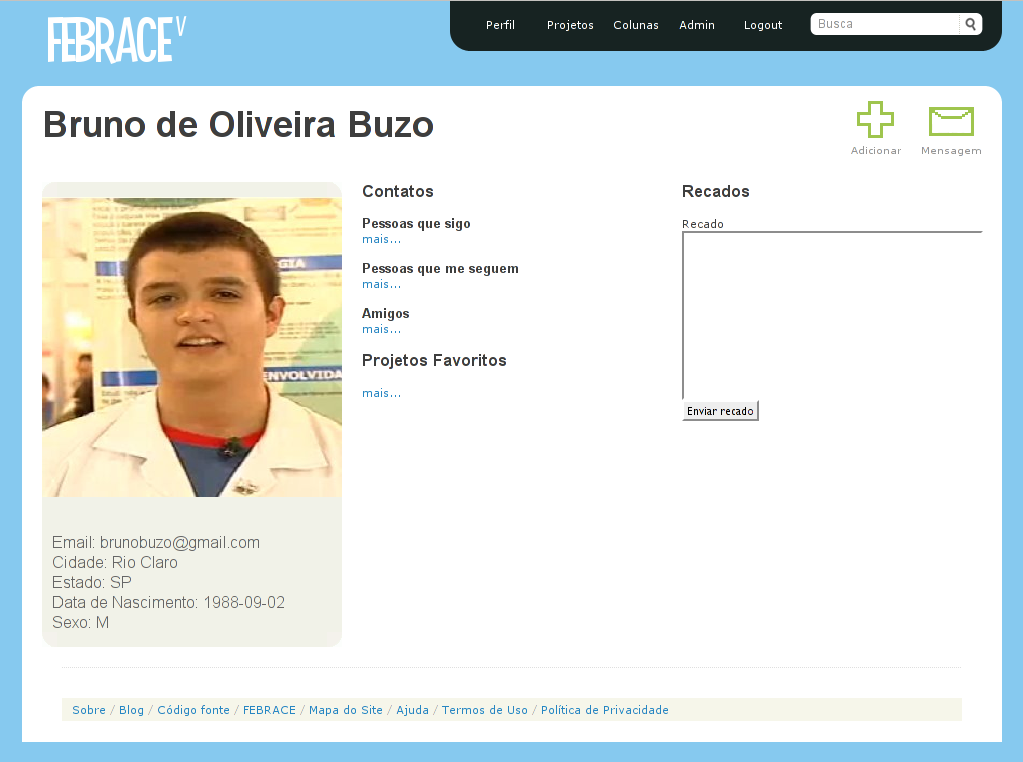
\includegraphics[width=0.7\linewidth]{arquivos/perfil.png}
        \end{center}
        \caption{Página de perfil de usuário}
        \label{perfil}
    \end{figure}

    \subsubsection{História 22 - Interface administrativa}
      O framework Django conta com uma interface administrativa padrão, que apresenta funcionalidades de criação, edição, visualização e deleção de quaisquer objetos do sistema que tenham sido cadastrados nessa interface, e pode ser personalizada para atender às diferentes necessidades de cada projeto. Na primeira iteração essa interface foi ativada e configurada para funcionar com a Febrace\textsuperscript{V}.

      Somente usuários com status de Administrador podem acessar essa funcionalidade.

  \subsection{Implementação da segunda iteração}
    A segunda iteração, com duração de duas semanas, de 11 a 22 de maio, teve como resultado a implementação das quatro histórias descritas à seguir:

    \subsubsection{História 7 - Visualização de projeto}
      Cada projeto cadastrado no sistema tem uma página no sistema, a partir da qual podem ser acessadas diversas de suas informações. Essa página também oferece links para a página da edição da Febrace que ele participou e para a página da categoria na qual está cadastrado, bem como para as páginas referentes às suas palavras-chave.

      Os demais elementos presentes na página de projetos são descritos em outros cartões relacionados ao tema.

    \subsubsection{História 8 - Listar participantes de um projeto}
      Cada projeto está associado aos usuários de seus participantes, alunos e orientadores. Esses participantes são mostrados na página de seu projeto, e suas representações (fotos ou nomes) são links para as páginas de perfil desses usuários.

    \subsubsection{História 9 - Suporte a vídeo no projeto}
      Outro elemento que pode estar associado a um projeto é um vídeo. Caso o projeto tenha um vídeo cadastrado, um \textit{player} é carregado na sua página, e o visitante desse projeto tem a opção de assistir a esse vídeo.

      Os vídeos da Febrace estão, até o presente momento, hospedados no portal IPTV Experimental\footnote{http://iptv.usp.br} da USP, e seu \textit{player} embarcado (\textit{embedded player}) é carregado junto às páginas do Febrace\textsuperscript{V}. Para visualizá-lo, o usuário precisa ter instalado em seu \textit{browser} um \textit{plugin} que o permita assistir um \textit{streaming} de vídeo no formato WMV (Windows Media Video). Há \textit{plugins} desse tipo para a maioria dos sistemas operacionais, incluindo Linux, MacOs e Windows.

      Se os vídeos da Febrace forem hospedados em outro serviço (como o YouTube\footnote{http://www.youtube.com} ou o Vimeo\footnote{http://www.vimeo.com}), alterações muito simples no sistema permitem adaptá-lo para esses casos.

    \subsubsection{História 24 - Gerenciamento de usuários no admin}
      É possível criar, editar, visualizar e apagar usuários pela interface administrativa. O mesmo se aplica aos modelos referentes a perfis. Nessa interface é também possível editar as permissões desse usuário, bem como seu status no sistema (ativo/inativo, administrador/usuário comum, etc.).

  \subsection{Implementação da terceira iteração}
    A terceira iteração foi realizada na quinzena de 25 de maio a 5 de junho. Nela foram implementadas as sete histórias à seguir:

    \subsubsection{História 13 - Amigos}
      Um aspecto muito importante das redes sociais é a possibilidade da criação de associações entre os usuários, e essa funcionalidade é oferecida na Febrace\textsuperscript{V}. Escolheu-se por adotar um modelo de associação baseado em "seguidores", tais como em redes como o Twitter\footnote{http://www.twitter.com} e o Stoa\footnote{http://stoa.usp.br}. Nesse modelo, um usuário não precisa solicitar a associação a um outro usuário, simplesmente escolhe seguí-lo. O usuário seguido pode ou não retribuir a associação. Caso o faça, surge a possibilidade da troca de mensagens privadas entre eles.

      No sistema desenvolvido um usuário autenticado, ao visitar a página de perfil de algum outro usuário, tem a opção de adicionar esse usuário como um amigo, selecionando o botão “Adicionar" presente em sua página.

      De volta à sua página, o usuário pode ver listados todas as pessoas que ele segue (perfis que ele selecionou como amigo), todas as pessoas que o seguem (pessoas que adicionaram seu perfil como amigo) a todas as relações mútuas (pessoas que o seguem e que são seguidas por ele).

      A qualquer momento ele pode deixar de seguir um usuário qualquer. Para isso, deve visitar o perfil desse usuário e selecionar a opção “Remover".

    \subsubsection{História 14 - Projetos prediletos}
      Um usuário autenticado pode também escolher quais são seus projetos prediletos na Febrace\textsuperscript{V}. As operações de adição ou remoção de um projeto predileto funcionam de maneira análoga à adição ou remoção de amigos. Ao visitar a página de um projeto, um usuário pode adicioná-lo como predileto clicando em “Adicionar". Se quiser desfazer a associação, deve visitar novamente a página desse projeto e clicar em “Remover".

      É mostrado no perfil de um usuário quais são seus projetos prediletos. Da mesma forma, é mostrada na página de um projeto a lista de usuários que o tem como predileto.

    \subsubsection{História 25 - Gerenciamento de conteúdo no admin}
      Além do gerenciamento de usuários e perfis (descrito na história 24), a interface administrativa pode ser utilizada para a gerencia de quaisquer outros conteúdos, como pode ser visto na figura~\ref{admin}. No momento, é possível por essa interface criar, editar, visualizar e remover os seguintes tipos de objetos:

      \begin{multicols}{3}
      \begin{itemize}
        \item{Comentários}
        \item{Páginas planas}
        \item{Links de amizade}
        \item{Instituições}
        \item{Links de prêmios}
        \item{Prêmios}
        \item{Projetos}
        \item{Links de projetos}
        \item{Tags}
        \item{Associação de Tags}
      \end{itemize}
      \end{multicols}

    \begin{figure}[h]
        \begin{center}
    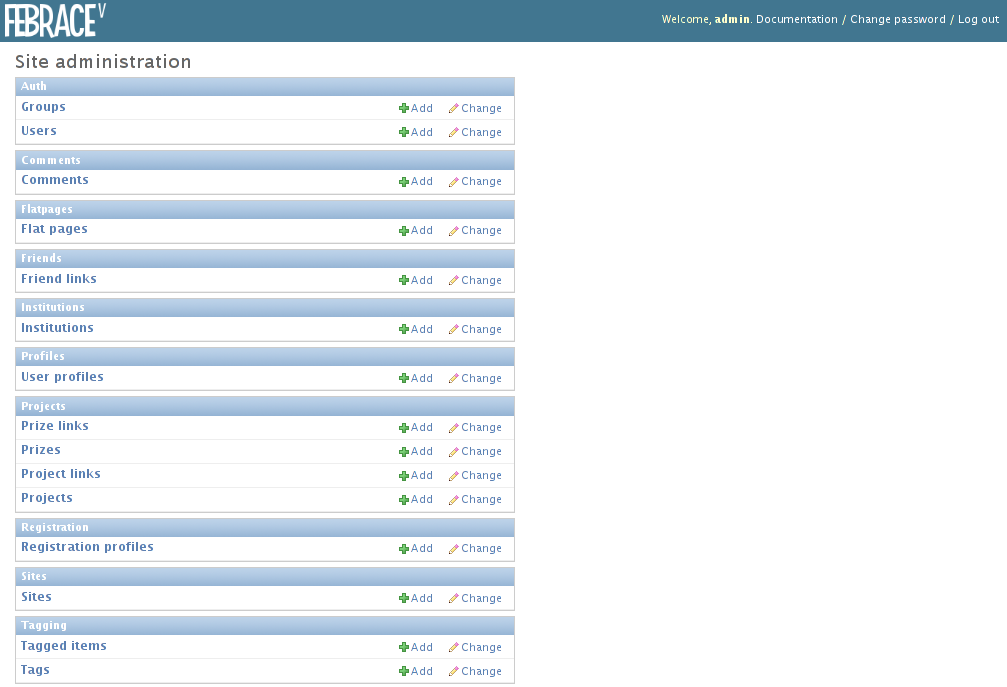
\includegraphics[width=0.7\linewidth]{arquivos/admin.png}
        \end{center}
        \caption{Interface administrativa do Febrace\textsuperscript{V}}
        \label{admin}
    \end{figure}

    \subsubsection{História 27 - Prêmios}
      Cada prêmio oferecido na Febrace tem sua página no sistema. Nessa página, além da descrição do prêmio, são listados todos os projetos que, em diferentes edições da Febrace, foram contemplados com ele. O vínculo de um prêmio a um projeto deve ser feito na interface administrativa.

    \subsubsection{História 28 - Instituições}
      Também as instituições (escolas, institutos, empresas patrocinadores, etc.) tem páginas com suas informações no sistema. Caso seja uma instituição que tenha levado alunos para expor projetos na Febrace, é disponibilizada em sua página a lista de projetos daquela instituição.

    \subsubsection{História 36 - Suporte a tags}
      Quaisquer objetos do sistema podem ser marcados com \textit{tags}, ou palavras-chave. As \textit{tags} tem por função, desse modo, agregar diferentes tipos de conteúdos sob categorias.

      As \textit{tags} podem ser inseridas pela interface administrativa, ou podem ser criadas diretamente ao serem utilizadas para marcar um objeto pela primeira vez.

      No momento, as \textit{tags} marcam apenas projetos e colunas, mas serão utilizadas para marcar outros conteúdos, como entradas de um diário de bordo.

  Esse cartão não planejado no levantamento inicial de histórias.

    \subsubsection{História 35 - Criação de páginas estáticas}
      A maioria das páginas que compõe a Febrace\textsuperscript{V} são dinâmicas, ou seja, são renderizadas conforme um contexto e uma requisição específicos. Há um conjunto de páginas, porém, que tem seus conteúdos e formas de exibição sempre iguais. Algumas das páginas do sistema são estáticas, como as páginas de “Mapa do site" e de “Termos de Uso".

      Há no \textit{framework} uma aplicação que facilita a criação e organização dessas páginas estáticas (páginas planas), que foi instalado e configurado para prover as páginas planas necessárias ao projeto.

  Esse cartão não planejado no levantamento inicial de histórias.

  \subsection{Implementação da quarta iteração}
    A quarta iteração, com duração de duas semanas, foi realizada entre 8 e 19 de junho, e teve como resultado a implementação de dez histórias. A descrição de cada uma delas é feita abaixo.

    \subsubsection{História 6 - Cancelamento de cadastro}
      Um usuário que não deseja mais fazer parte da rede social pode solicitar a remoção de seu perfil do sistema. Para isso, uma vez autenticado deve selecionar a opção de edição de perfil e, na página de edição, selecionar apagar conta. Caso realmente deseje apagar a conta, o usuário deverá confirmar novamente a opção.

      Dessa maneira, o perfil do usuário e quaisquer conteúdos ligados a ele serão removidos. Conteúdos gerados por esse usuário em outros lugares do sistema (comentários em projetos, por exemplo) serão porém mantidos.

    \subsubsection{História 10 - Visualização dos prêmios de um projeto}
      Na página de detalhes de um projeto são listados os prêmios que esse projeto ganhou na edição da Febrace em que participou. Ao clicar nos prêmios, tem-se acesso a sua página de detalhes, descrita na História 27.

    \subsubsection{História 20 - Colunas}
      Membros da equipe da Febrace contam com uma região do sistema na qual podem, sempre que quiserem, criar textos que desejem ser compartilhados com os outros integrantes da rede social. É a sessão de colunas, que pode ser lida e comentada por qualquer usuário, autenticado ou não.

    \subsubsection{História 16 - Recados/Caixas de comentários}
      Um dos componentes das páginas de perfil de usuário é o mural de recados. Nele, outros usuários podem deixar pequenas mensagens de texto para o dono do perfil. Os recados podem ser tanto escritos por usuários autenticado quanto por visitantes. No caso de um usuário autenticado, o recado é automaticamente vinculado a ele. No caso de um visitante, é solicitado o preenchimento de um pequeno formulário contendo nome e email válido.

      A mesma funcionalidade é oferecida nas páginas de projeto.

    \subsubsection{História 18 - Busca}
      Há no menu principal do site uma ferramenta de busca. Ao se digitar um texto e selecionar o botão enviar, o sistema realiza a busca dos termos procurados, e devolve uma página com elementos que atendam a essa requisição. No momento, a busca retorna três tipos de objetos: projetos, perfis de usuário e \textit{tags}. O sistema poderá ser expandido futuramente para suportar outros tipos de objetos.

      A sintaxe da busca é semelhante à de mecanismos de busca como o Google, por exemplo. Se mais de um elemento for inserido, a busca procura ocorrências dos termos simultâneamente, em qualquer ordem. Termos envoltos por aspas duplas são procurados tal como digitados, na ordem e em ocorrência simultânea.

    \subsubsection{História 30 - Interface de escrita de colunas}
      Para que os membros da Equipe da Febrace possam criar novos textos para a seção de colunas, eles devem acessar a interface administrativa. Lá eles contam com uma ferramenta que os permitem editar seus textos e gerenciar textos escritos anteriormente.

    \subsubsection{História 32 - Preenchimento dos bancos de dados}
      Para a apresentação do projeto, foi necessário popular o banco de dados do sistema com projetos de edições anteriores da feira. Buscou-se incluir no sistema projetos de categorias variadas, priorizando-se os projetos que tenham sido premiados na feira. A entrada desses dados foi realizada manualmente.

  Esse cartão não planejado no levantamento inicial de histórias.

    \subsubsection{História 34 - Home page}
      Foi criada a \textit{homepage} para o projeto (figura~\ref{homepage}), que apresenta cinco sessões principais. A primeira é o menu presente em todas as outras páginas, pelo qual é possível cadastrar-se, realizar o login, realizar buscas ou acessar algumas sessões do site. Outra é o conjunto de textos que explicam a finalidade do Febrace\textsuperscript{V} e convidam o visitante a conhecer mais a respeito. Em seguida temos uma sessão com notícias e outras atividades recentes. No rodapé, tem-se acesso ao conjunto de páginas estáticas (mapa, termos de uso, etc.) e a outros sites ligados ao sistema, como o blog do desenvolvimento, o repositório de código e a página da Febrace. No centro da página, tem-se acesso a um projeto ou conteúdo de destaque.

  Esse cartão não havia sido planejado no levantamento inicial de histórias.

    \begin{figure}
        \begin{center}
    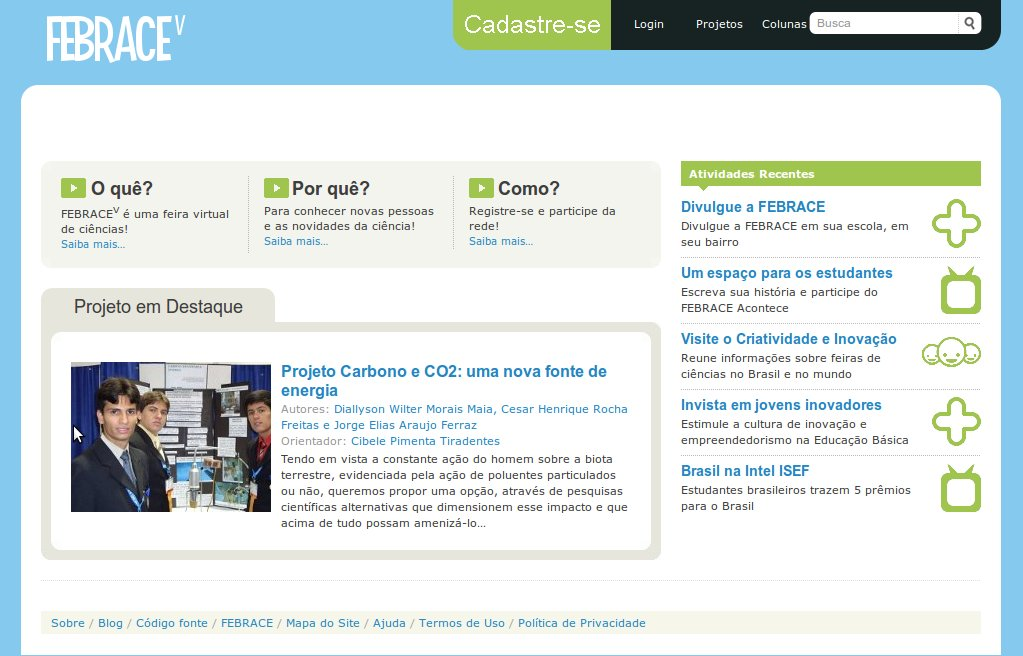
\includegraphics[width=0.7\linewidth]{arquivos/home.png}
        \end{center}
        \caption{Página principal do Febrace\textsuperscript{V}}
        \label{homepage}
    \end{figure}

    \subsubsection{História 31 - Listagens}
      A maioria dos objetos presentes no sistema tem páginas individuais, como é o caso de projetos, perfis, instituições, prêmios e \textit{tags}. Para que a navegação seja consistente, entretanto, não basta que só os objeto tenham suas páginas relativas, sendo necessário que cada grupo de objetos tenha uma página agregadora. Por isso foram desenvolvidas as páginas de listagem.

      Para perfis, prêmios, instituições e \textit{tags}, as páginas de listagem operam de maneira análoga, gerando listas com os nomes de todos os objetos daquele grupo, com o respectivo \textit{link} para sua página de detalhes. Para projetos o funcionamento é um pouco diferente. São disponibilizadas, nesse caso, dois tipos distintos de listagem, um que agrega projetos conforme a edição da Febrace em que participaram, outro que os agrega conforme sua categoria.

      Um caso particular é a página de detalhes de uma \textit{tag}, que é também uma listagem, dos elementos que foram marcados por essa \textit{tag}.

  Esse cartão não havia sido planejado no levantamento inicial de histórias.

    \subsubsection{História 33 - Criação de \textit{templates}}
      \textit{Templates} são os componentes que determinam a apresentação do projeto, e por eles definem-se quais componentes estarão presentes em quais páginas, e de que forma.

      Para evitar a repetição de código, os \textit{templates} foram organizados seguindo uma hierarquia. Elementos presentes em todas as páginas, como o menu principal, o logotipo e o rodapé das páginas, estão definidos em um template na base dessa hierarquia. Seguindo o paradigma de orientação a objetos, esse \textit{template} base é herdado pelos outros templates. Caso haja atributos presentes nele que não são desejados nos herdeiros, eles podem redefinir a implementação, reescrevendo ou estendendo os elementos herdados.

  Esse cartão não planejado no levantamento inicial de histórias.
